% LaTeX Article Template - customizing header and footer
\documentclass{article}

\newtheorem{thm}{Theorem}

% Set left margin - The default is 1 inch, so the following 
% command sets a 1.25-inch left margin.
\setlength{\oddsidemargin}{0.25in}

% Set width of the text - What is left will be the right margin.
% In this case, right margin is 8.5in - 1.25in - 6in = 1.25in.
\setlength{\textwidth}{6in}


% Set top margin - The default is 1 inch, so the following 
% command sets a 0.75-inch top margin.
\setlength{\topmargin}{-0.25in}

% Set height of the header
\setlength{\headheight}{0.3in}

% Set vertical distance between the header and the text
\setlength{\headsep}{0.2in}

% Set height of the text
\setlength{\textheight}{9in}

% Set vertical distance between the text and the
% bottom of footer
% Set the beginning of a LaTeX document
\usepackage{multirow}
\usepackage{fullpage}
\usepackage{graphicx}
\usepackage{amsthm}
\usepackage{amssymb}
\usepackage{algpseudocode}
\usepackage{tikz-qtree}
\usepackage{qtree}
\usepackage{amsmath}



\graphicspath{ {images/} }


\begin{document}\title{CSCI-B657: Computer Vision \\Assignment 1: Image Processing and Recognition Basics}         % Enter your title between curly braces
	\author{Sumit Kumar Dey (skdey@indiana.edu) \\ Prakash Rajagopal (prakraja@indiana.edu) \\Raghuveer Krishnamurthy Kanchibail (rkanchib@iu.edu)\\ \\Due date: February 9th 2016}        % Enter your name between curly braces
	\date{\today}          % Enter your date or \today between curly braces
	\maketitle
	
	\makeatother
	
	\pagestyle{plain}
	\begin{enumerate}
		\item Implement a function that convolves a greyscale image I with an arbitrary two-dimensional kernel H.
		(You can use a brute-force implementation – no need to use Fourier Transforms, although you can if you want.) Make sure your code handles image boundaries in some reasonable way \\ \\
		\textbf{Solution:}
		\begin{enumerate}
			\item We have implemented the convolution function by Brute force method.
			\item Convultion is achieved by using the formula: \\G[i,j] = $\sum\limits_{u=-k}^k \sum\limits_{v=-k}^k H[u,v] F[i-u,j-v]$ 
			\item We have made use of 4 for-loops in order to convolve an image
			\item Image boundaries have been handled by padding 0's
			\item The run-time of this brute force implementation is O(p.q) where p is the complexity required to iterate through the image matrix which is $O(n^2)$ and q is the complexity for iterating the kernel matrix which is $O(n^2)$, where r is the size of the kernel matrix.
			
			\item The below images show the  result of convolving a greyscale image. \\ \\
			\begin{center}
				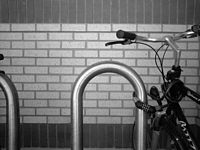
\includegraphics{Bikesgray.png} \\
				Figure a. Original Image
			\end{center}
			\begin{center}
				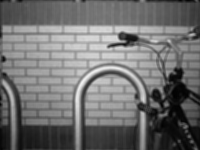
\includegraphics{detected_test.png}	\\	
				Figure b. Blurred image after applying a 3x3 mean filter \\
			\end{center} 
		\end{enumerate}
		
		\item Implement a function that convolves a greyscale image I with a separable kernel H. Recall that a separable kernel is one such that H = ${h^T}_x h_y$, where $h_x$ and $h_y$ are both column vectors. Implement efficient convolution by using two convolution passes (with $h_x$ and then $h_y$), as we discussed in class. Make sure your code handles image boundaries in some reasonable way \\ \\
		\textbf{Solution:}
		\begin{enumerate}
		\item We have implemented the convolution function by Brute force method.
		\item Convolution here is achieved by separating the kernel into row and column kernels.
		\item Valid row and column kernels should be passed in order to convolve an image.
		\item The image is first convolved with a row filter and the resulting image is then convolved with column filter. Doing so, reduces the computation steps significantly.
		\item The run-time of this brute force implementation is O(p+q) where p is the complexity for the convolution of image with a row filter which $O(n^3)$ and q is the complexity for the convolution of the resulting image with the column filter which is $O(n^3)$
		\item Image boundaries are handled by reflecting the values at the opposite sides of the image.
		\item The below images show the  result of convolving a greyscale image. \\ \\
		\begin{center}
			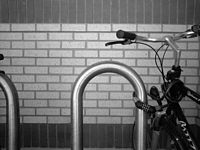
\includegraphics{Bikesgray.png} \\
			Figure a. Original Image
		\end{center}
		\begin{center}
			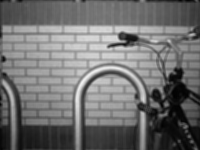
\includegraphics{detected_test.png}	\\	
			Figure b. Blurred image after convolving with a separable kernel \\
		\end{center}   
		\end{enumerate}
		\item A main goal of OMR is to locate various musical symbols in the image. Suppose for each of these
		symbols, we have a black and white “template” – a small m×n-pixel image containing just that symbol
		– with black pixels indicating the symbol and white pixels indicating background. Call this template
		T. Now we can consider each m × n-pixel region in the image of a sheet of music, compute a score
		for how well each region matches the template, and then mark the highest-scoring ones as being the symbol of interest. In other words, we want to define some similarity function ${f^I}_T$
		(i, j) that evaluates how similar the region around coordinates (i, j) in image I is to the template. \\ One could define this function f(·) in many different ways. One simple way of doing this is to simply count the number of pixels that disagree between the image and the template – i.e. the Hamming distance between the two binary images, \\ \\
		${f^I}_T$(i, j) =$\sum\limits_{k=0}^{m-1} \sum\limits_{l=0}^{n-1}$ I(i + k, j + l)T(k, l) + (1 - I(i + k, j + l))(1 - T(k, l)) \\ \\ This function needs to be computed for each m × n-pixel neighborhood of I. Fortunately, with a small amount of manipulation, this can performed using a convolution operation!\\
		Implement a routine to detect a given template by doing the convolution above. When a note is
		detected, it should also estimate the pitch of the note (i.e. letter between A and G). To help you get started, we’ve supplied an easy test image (music1.png) and three templates (template1.png, template2.png,
		template3.png). Your program should generate an output image similar to the one in
		Figure 1(b) showing the symbols that have been detected.\\ \\
		\textbf{Solution:} \\
		We are detecting the musical symbols present in the music1.png by comparing it with all templates provided. 
		Below is the image of the music1.png provided to us. 
		\begin{center}
			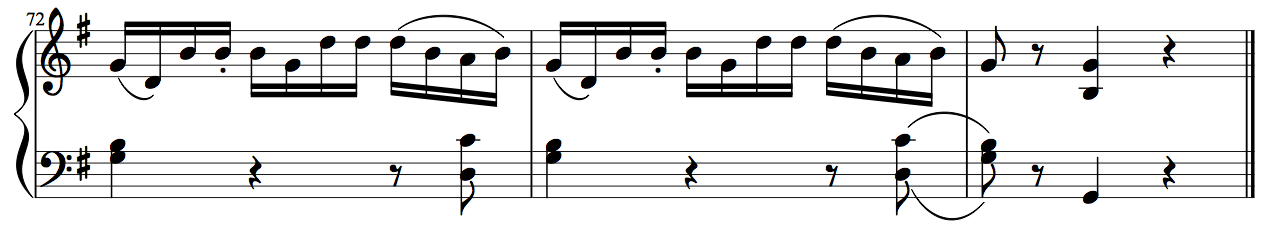
\includegraphics[height=3cm,width=14cm ]{music1.png}	\\	
			Figure a. music1.png \\ 
		\end{center}   
		The music1.png will be our input to the $detect\_image$ function along with the list of templates, the line temp image and the symbols. \\
		The $detect\_image$ function then computes the hamming distance between each of the templates and the image. \\
		The hamming distance between the input file and the template is found out by making use of the formula: \\
		$\sum\limits_{k=0}^{m-1} \sum\limits_{l=0}^{n-1}$ I(i + k, j + l)T(k, l) + (1 - I(i + k, j + l))(1 - T(k, l)) \\ \\
		This is achieved by making use of 4 for-loops and convolving both the images with each other and adding them. \\
		The resultant output is then sent to the function $find\_match\_and\_push\_to\_vector$ \\ \\
		The $find\_match\_and\_push\_to\_vector$ function first calculates the maximum hamming distance between the input file and the template.We have applied heuristics and any value between max and max - heuristic value is considered as a perfect match. Once the prefect match is found out, appropriate boxes are drawn on appropriate notes in the music file. \\
		The below image shows the result after drawing boxes for music1.png. \\
		 	\begin{center}
		 		
\includegraphics[height=3cm,width=14cm ]{detected.png}	\\	
		 		Figure b. Results after finding the musical symbols in music1.png \\ 
		 	\end{center}
		\item An alternative approach is to define the template matching scoring function using edge maps, which
		tend to be less sensitive to background clutter and more forgiving of small variations in symbol appearance.
		To do this, first run an edge detector on the template and the input image. You can use the
		Sobel operator and your separable convolution routine above to do this. Then, implement a version of
		template matching that uses the following scoring function: \\
		${f^I}_T$(i, j) =$\sum\limits_{k=0}^{m-1} \sum\limits_{l=0}^{n-1}$ T(k,l) min $a_{\in [0,m)}$ min $b_{\in [0,m)}$ $\gamma (I(i + a, j + b)) + \sqrt{(a − k)^2 + (b − l)^2}$ \\
		where I and T here are assumed to be edge maps, having value 1 if a pixel is an edge and 0 otherwise,and $\gamma(\cdot)$ is a function that is 0 when its parameter is non-zero and is infinite when its parameter is 0. \\
		Note that computing this scoring function for every pixel in the image can be quite slow if implemented
		naively. Each of the min’s involves a nested loop, each summation involves a nested loop, so computing
		the score for every pixel (i, j) requires a sextuply-nested loop! However, we can once again use a simple
		instance of dynamic programming to speed up this calculation. Notice that the above equation can be
		re-written as:\\
		${f^I}_T$(i, j) =$\sum\limits_{k=0}^{m-1} \sum\limits_{l=0}^{n-1}$ T(k, l) D(i + k, j + l) \\ where \\ \\ D(i,j) = min $a_{\in [0,m)}$ min $b_{\in [0,m)}$ $\gamma (I(a,b)) + \sqrt{(i - a)^2 + (j - b)^2}$ \\ \\
		and M × N are the dimensions of I. Notice that D(i, j) has an intuitive meaning: for every pixel
		(i, j), it tells you the distance (in pixels) to the closest edge pixel in I. More importantly, notice that
		re-writing the equations in this way reduces the number of nested loops needed to compute ${f^I}_T$
		from six to four, because D can be pre-computed. Computing D for all pixels requires four nested loops if implemented naively, but requires only quadratic time if you’re clever. \\ \\
		\textbf{Solution:} \\ \\
		In the alternate approach, we are detecting the musical symbols present in the music1.png by comparing it with all templates provided. 
		Below is the image of the music1.png provided to us. 
		\begin{center}
			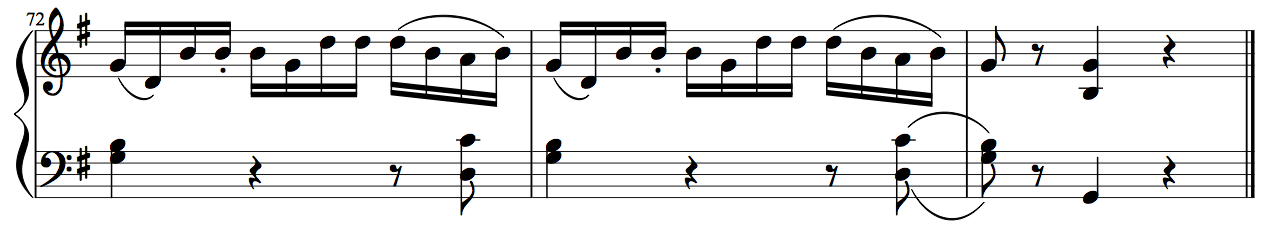
\includegraphics[height=3cm,width=14cm ]{music1.png}	\\	
			Figure a. music1.png \\ 
		\end{center}   
		The music1.png will be our input to the $detect\_image2$ function along with the list of templates, the line temp image and the symbols. \\
		The $detect\_image2$ function first applies the non-maximum suppression on the input image. This is achieved by passing the input image along with a low threshold value(0) and high threshold value(3) to the $find\_edges\_non\_max\_supr$  \\
		The $find\_edges\_non\_max\_supr$ function then convolves the input image with the sobel gradient filter to get the 2 derivatives. One for the changes in the x-direction and one for the y-direction. The two derivatives will be used to calculate the gradient magnitude. The gradient magnitude is computed by sending the two derivatives to $compute\_grad\_magnitude$ \\
		Since we have the gradient magnitude and the two image derivatives, we will send these to \\ $perform\_nms\_suppression\_using\_gradient$. This function calculates the neighboring boundaries in all the 8 directions. Then we call the $apply\_hysteresis\_threshold$ function to preserve any weak edges present within the 8 neighboring pixels. The resultant is then sent to $get\_distance\_to\_closest\_edge$. The output from the $get\_distance\_to\_closest\_edge$ will now have all the strong edges which is nothing but, \\ D(i,j) = min $a_{\in [0,m)}$ min $b_{\in [0,m)}$ $\gamma (I(a,b)) + \sqrt{(i - a)^2 + (j - b)^2}$ of the equation \\ ${f^I}_T$(i, j) =$\sum\limits_{k=0}^{m-1} \sum\limits_{l=0}^{n-1}$ T(k, l) D(i + k, j + l)
		\\ Each template then undergoes non-maximum suppression and is compared with D(i,j) using the function $get\_template\_match$. The $get\_template\_match$ implements the scoring function \\ ${f^I}_T$(i, j) =$\sum\limits_{k=0}^{m-1} \sum\limits_{l=0}^{n-1}$ T(k, l) D(i + k, j + l)\\
		This is then passed to $find\_match\_and\_push\_to\_vector2$. We now calculate the minimum score between the input image and the template. We have applied heuristics to find the number. Any value between min and min + heuristic value is said to be a match and an appropriate box is drawn for the matched image. This is achieved with a complexity of $O(n^2)$ \\
		\begin{center}
			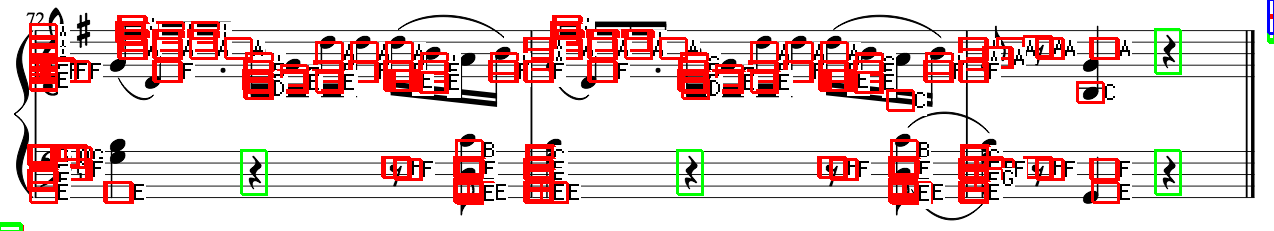
\includegraphics[height=3cm,width=14cm ]{detected5.png}	\\	
			Figure b. Results after finding the musical symbols in music1.png \\ 
		\end{center}
		
		\item
		The sample image and template we provided above were carefully designed so that the size of the
		template exactly matched the size of the objects appearing in the image. In practice, we won’t know
		the scale ahead of time and we’ll have to infer it from an image. Fortunately, if we can find the staff
		lines, then we can estimate the note head size, since the distance between staff lines is approximately the
		height of a note head. To find the staves, one could first find horizontal lines using Hough transforms
		and then try to find groups of five equally-spaced lines, but this two-step approach introduces the
		possibility of failure: if a line is not detected properly, an entire staff might not be found. A better
		approach is to apply the Hough transform to find the groups of five lines directly.
		Implement a Hough transform to do this. Assume that the lines in the staves are perfectly horizontal,
		perfectly parallel, and evenly spaced (but we do not know the spacing ahead of time). Then the Hough
		voting space has two dimensions: the row-coordinate of the first line of the staff, and the spacing
		distance between the staff lines. Each pixel in the image then “votes” for a set of row-coordinates
		and spacing parameters. Each peak in this voting space then corresponds to the row-coordinate and
		spacing of a staff line, which in turn tells us where each of the five lines of the staff is located. \\ \\
		\textbf{Solution:} \\ \\
		To detect the staves in the input image we are making use of the Hough transform. The process starts with a call to the $start\_hough$ function. The $start\_hough$ takes a noiseless image(noiseless image is produced by convolving our input image with a gaussian filter), low threshold, high threshold, maximum number of lines and the voting threshold count as the parameters. \\
		The $start\_hough$ function then calls the $find\_edge\_non\_max\_supr$ by passing the noiseless image, low threshold, high threshold, and the maximum value for a pixel(we have taken the value to be '3'). Now we obtain an edge image having only strongly connected edges \\
		Now this image is sent as a parameter for the function $hough\_transform$. The $hough\_transform$ function transforms the image and maps it into polar co-ordinates. The accumulator is filled with the polar co-ordinates. The size of the accumulator is taken to be $max\_radius(maximum~ radius = \sqrt{2} * max(height,width)$) to 180.The value $\rho$ is calculated for each degree from 90-180 by using: \\
		$\rho = xcos\theta + ysin\theta$ \\
		The accumulator is filled with votes for each value of $[\rho][\theta]$ \\
		The accumulator looks as follows: \\
		\begin{center}
			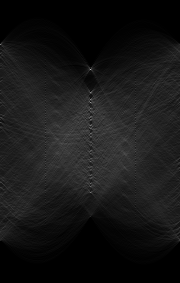
\includegraphics[height=8cm, width = 3cm]{detectacc.png} Figure a.~~~~~~~~~~~~~~~~~~~~~
			
\includegraphics [height=8cm, width = 3cm]{detectacc1.png} Figure b.\\ 	
			Figure a. Image of the accumulator in hough space with $\theta$ = 0-180 \\ 
			Figure b. Image of the accumulator in hough space with $\theta$ = 90 -180\\ 
		\end{center}
		
		Once we have the number of votes in our accumulator, we can transform them into x-y plane to filter out the lines which are below threshold count. We have applied a heuristic to find out the minimum number of lines which is possible by taking out the minimum value among [minimum number of lines specified, number of lines available, the size of the accumulator and user passed threshold of voting count]\\
		We have made use of priority queue to store the $[\rho,\theta]$ pair in increasing order. These 
		$[\rho,\theta]$ pair are then mapped back into the x-y plane. To accommodate lines which are slant, we have made use of heuristic which allows us to consider lines with an error of 2/90 degree. The resulting image will be as follows:
		\begin{center}
			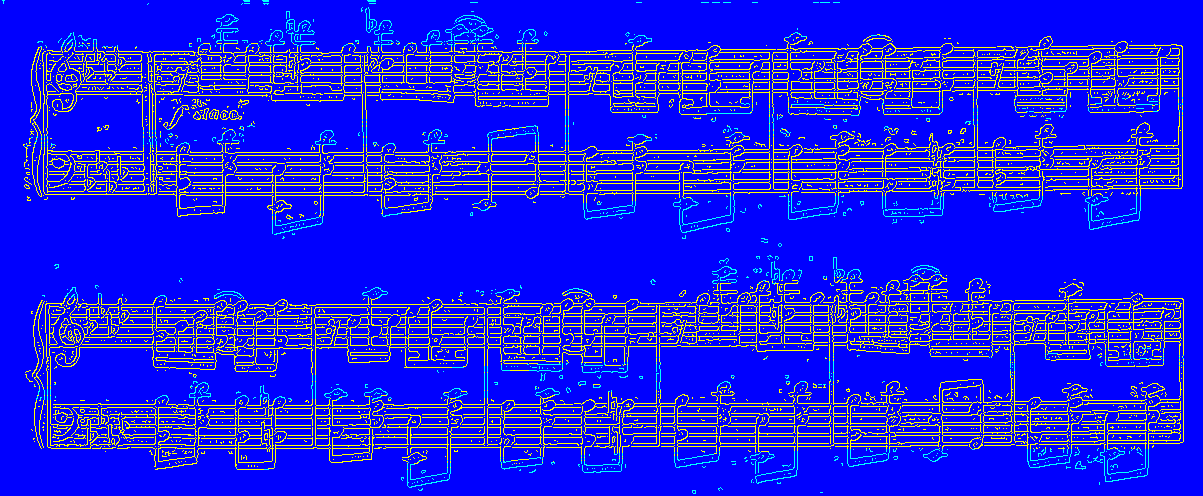
\includegraphics[height=3cm,width=14cm ]{detect_hough.png}	\\
			Figure c. Hough transform applied to music1.png\\ 
		\end{center}
		\begin{center}
			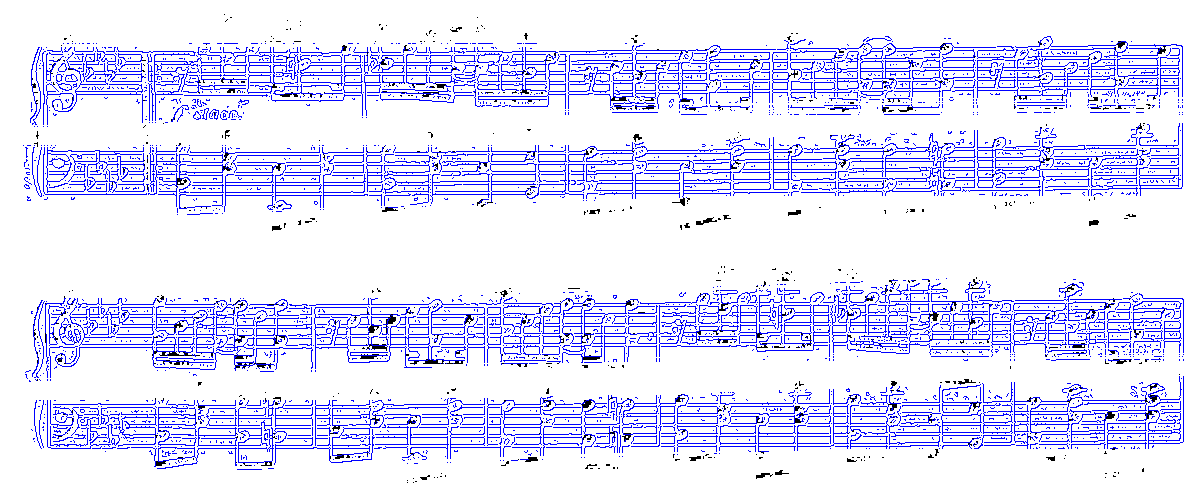
\includegraphics[height=3cm,width=14cm ]{staves.png}	\\
			Figure d. Final output with blue lines indicating the staves in music4.png\\ 
		\end{center}
		\item
		Now combine the above techniques together to implement a simple OMR system. In this assignment, we’ll focus on just detecting the staves and the three symbols shown in Figure 1(a): filled-in note heads,quarter rests, and eighth rests. In particular, your assignment should do the following:
		\begin{enumerate}
			\item 
			Load in a specified music image.
			\item
			Detect all of the staves using step 6 above. In addition to giving you the staves, this also gives
			an estimate of the scale of the image - i.e. the size of the note heads - since the space between staff lines is approximately the height of a notehead.
			\item Rescale the image so that the note head size in the image agrees with the size of your note head
			templates. (Alternatively, you can rescale the note templates so that they agree with the image,
			you can have a library of pre-defined templates of different scales and select the appropriate one
			dynamically.)
			\item Detect the notes and eighth and quarter rests in the image, using the approach of step 4, step
			5, some combination, or a new technique of your own invention. The goal is to correctly find as many symbols as possible, with few false positives. \\ \\
			\textbf{Solution:} \\ \\ \\ \\
			We have made use of $start_hough$ function to detect all the staves of the image. Now we get the distance between staffs. We also get the size of note head and since the input image has the height between staffs. Using this informations we get the scale that we need to vary for each template and using the respective generated scale template we calculate the hamming distance that gives highest difference between average hamming score and the maximum hamming score in a reasonable range to decide the position of corresponding template. We have made use of ensemble methods to make use of ${80\%} $ of the step 4 and ${20\%}$ of the step 5 to detect the notes and quarter rests in the image. We have tried a brute force method to find magnification using template 1 wherein we get the hamming distance and determine using a heuristic if the template gives the best possible match for a given scale. This heuristic depends on the normalized difference between average and max value in hamming result. According to this, the maximum difference indicates a steeper graph in the curve - therefore the template at that scale provides us the best possible match. Using this scale, the remaining templates are scanned and detected.
		\end{enumerate}
	\end{enumerate}
\end{document}